\ifdefined \buildingFullOPALManual \else


%\ifx \@buildingFullOPALManual \@empty
%\else

%\documentclass[12pt,a4paper]{report}
\documentclass[a4paper]{book}

%% does not work in Latex2Html mode
%\usepackage{hyperref}

\usepackage[T1]{fontenc}
\usepackage{url}
\usepackage{html}
\usepackage{epic}
\usepackage{eepic}
\usepackage{makeidx}
\usepackage{array}
\usepackage{times}
\usepackage{amsmath}
\usepackage{amsxtra}
\usepackage{bm}
\usepackage[thin,thinp,thinc]{esdiff}
\usepackage{etoolbox}
\usepackage{graphicx}
\usepackage{dingbat}
\usepackage{color}
\usepackage{subfig}
\usepackage{boxedminipage}
\usepackage{alltt}
\usepackage{nicefrac}
\usepackage{calc}
%\usepackage{pdfdraftcopy}             % Draft
\usepackage{tikz}
\usetikzlibrary{
  er,3d,calc,fadings,trees,positioning,arrows,chains,decorations.pathreplacing,
  decorations.pathmorphing,shapes,shapes.symbols,shapes.arrows,matrix,through,decorations.text
}

\tikzset{
  >=stealth',
  punktchain/.style={rectangle,rounded corners, draw=black, very thick,text width=10em,
                     minimum height=3em, text centered, on chain},
  line/.style={draw, thick, <-},
  element/.style={tape,top color=white,bottom color=blue!50!black!60!,minimum width=8em,
                  draw=blue!40!black!90, very thick,text width=10em, minimum height=3.5em,
                  text centered, on chain},
  every join/.style={->, thick,shorten >=1pt},
  tuborg/.style={decorate},
  tubnode/.style={midway, right=2pt}
}

\tikzstyle{material}=[draw, fill=blue!20, text width=16.0em, text centered, minimum height=1.5em]
\tikzstyle{diagramstep} = [material, text width=20em, minimum width=10em, minimum height=3em, rounded corners]
\tikzstyle{line} = [draw, thick, color=black!50, -latex']

\usepackage{booktabs}
\usepackage{xspace}
\usepackage{xstring}

\usepackage{fancyvrb}
\usepackage{rotating}
\usepackage{float}

\usepackage{tabularx}
\usepackage{longtable}
\setcounter{LTchunksize}{3}

\usepackage[section]{placeins}
\usepackage{MnSymbol}
\usepackage{microtype}
\usepackage{setspace}
\usepackage{dcolumn}

\usepackage[vmargin={3.0cm,3.0cm},
            hmargin={2.0cm,3.0cm}]{geometry}

\usepackage{upgreek}
\usepackage[binary-units=true]{siunitx}
\sisetup{exponent-product = \cdot,math-ohm=\Upomega,text-ohm=\ensuremath{\Upomega}}
\DeclareSIUnit{\clight}{c}
\DeclareSIUnit\gauss{Ga}

\usepackage{engord}
\usepackage{wasysym}
\DeclareSIUnit[number-unit-product = \,]{\permill}{\permil}

\usepackage{hyperref}
\hypersetup{
    pdftitle          = The OPAL Framework,
    pdfauthor         = {Andreas Adelmann, Achim Gsell, Valeria Rizzoglio, Christof Metzger-Kraus,
                         Yves Ineichen, Xiaoying Pang, Steve Russell, Chuan Wang, Jianjun Yang,
                         Suzanne Sheehy, Chris Rogers, Daniel Winklehner},
    pdfsubject        = User's Reference Manual,
    pdffitwindow      = true,               % page fit to window when opened
    pdfnewwindow      = true,               % links in new window
    colorlinks        = true,               % false: boxed links; true: colored links
    linkcolor         = black!80!green,     % color of internal links
    citecolor         = black!20!red,       % color of links to bibliography
    urlcolor          = blue,               % color of external links
    breaklinks        = true,
    bookmarksnumbered = true,
    plainpages        = false
}

\usepackage{ifthen}

\newif \iflinuxwindows
\linuxwindowstrue   % set this to true when building the manual on Linux or Windows
\iflinuxwindows
\usepackage{epstopdf}
\fi

\usepackage[backend=biber,
            style=phys,
            biblabel=brackets,
            maxnames=3,
            doi=true,
            isbn=true,
            url=true]{biblatex}
%---- macros ----

\renewcommand{\topfraction}{1.0}
\renewcommand{\bottomfraction}{1.0}
\renewcommand{\textfraction}{0.0}
\renewcommand{\arraystretch}{2.0}
\newenvironment{tex2html_nowrap}{}{}


\newcommand{\Newline}{\hfil \\}


\newsavebox{\ExampleBox}
\newenvironment{example}
 {\VerbatimEnvironment
  \begin{flushleft}
  \begin{lrbox}{\ExampleBox}
    \begin{minipage}{\linewidth}
  \begin{Verbatim}[frame=lines,xleftmargin=0cm,fontsize=\footnotesize,samepage=true]}
 {\end{Verbatim}
  \end{minipage}
  \end{lrbox}
  \mbox{\usebox{\ExampleBox}}
  \end{flushleft}
 }

\newenvironment{longexample}
{\Verbatim[frame=lines,xleftmargin=0mm,fontsize=\footnotesize]}
{\endVerbatim}

%\examplefromfile{filename} reads in a text file and displays it in the document.
\newcommand{\examplefromfile}[1]{
\VerbatimInput[frame=lines,xleftmargin=0mm,fontsize=\footnotesize,label=\texttt{#1}]{#1}}

%for upright d of differentials
\makeatletter
\newcount\my@repeat@count

\newcommand{\myrepeat}[2]{%
  \begingroup
  \my@repeat@count=\z@
  \@whilenum\my@repeat@count<#1\do{#2\advance\my@repeat@count\@ne}%
  \endgroup
}

\newcommand{\differential}[1]{\ifstrempty{#1}{\ES@dop\ES@difint}{\ES@dop^{#1}\ES@difint}}
\newcommand{\pdifferential}[1]{\ifstrempty{#1}{{\partial\,}}{{\partial^{#1}\,}}}

\makeatother

\newcommand{\der}[3][]{\frac{\differential{#1}#2}{\differential{}\ifstrempty{#1}{#3}{#3^#1}}}
\newcommand{\parder}[3][]{\frac{\pdifferential{#1}#2}{\pdifferential{}\ifstrempty{#1}{#3}{#3^#1}}}
\newcommand{\niceder}[3][]{\nicefrac{\differential{#1}#2}{\differential{}\ifstrempty{#1}{#3}{#3^#1}}}
\newcommand{\uglyder}[3][]{{\differential{#1}#2}/{\differential{}\ifstrempty{#1}{#3}{#3^#1}}}
\newcommand{\uglyparder}[3][]{{\pdifferential{#1}#2}/{\pdifferential{}\ifstrempty{#1}{#3}{#3^#1}}}
\newcommand{\dd}[1][]{\; \differential{#1}}
\newcommand{\primed}{^{\prime}}
\newcommand{\dprimed}{^{\prime\prime}}
\newcommand{\nprimed}[1]{^{\myrepeat{#1}{\prime}}}

%Editing Macros
\newcommand{\TODO}[1]{{\color{red}\ifthenelse{\boolean{ShowDebug}}{[TODO: #1]}{}}}



%text in gray box
\newsavebox{\fmbox}
\definecolor{lightgray}{gray}{0.95}
\newenvironment{fmpage}
   {\vspace{-1.0cm}\begin{lrbox}{\fmbox}\begin{minipage}[t]{13.5cm}\vspace{0.1cm}}
   {\vspace{-0.4cm}\end{minipage}\end{lrbox}\begin{center}\fcolorbox{black}{lightgray}{\usebox{\fmbox}}\end{center}}


% Definition new signes
\newcommand{\R}{{\mathbb R}} % real numbers
\newcommand{\Q}{{\mathbb Q}} % rational numbers
\newcommand{\Z}{{\mathbb Z}} % integer numbers
\newcommand{\N}{{\mathbb N}} % natural numbers

\newcommand{\mad}{\textsc{mad}\xspace}
\newcommand{\madnine}{\textsc{mad9}\xspace}
\newcommand{\madninep}{\textsc{mad9p}\xspace}
\newcommand{\madeight}{\textsc{mad8}\xspace}
\newcommand{\classic}{\textsc{classic}\xspace}

\makeatletter
\newcommand{\opal@impl}{\textsc{Opal}}
\newcommand{\opalt@impl}{\textsc{Opal-t}}
\newcommand{\opalcycl@impl}{\textsc{Opal-cycl}}
\newcommand{\opalmap@impl}{\textsc{Opal-map}}
\newcommand{\opalenv@impl}{\textsc{Opal-e}}

\newcommand{\opal}{\opal@impl\xspace}
\newcommand{\opalt}{\opalt@impl\xspace}
\newcommand{\opalcycl}{\opalcycl@impl\xspace}
\newcommand{\opalmap}{\opalmap@impl\xspace}
\newcommand{\opalenv}{\opalenv@impl\xspace}

\newcommand{\noopalt}{\leftthumbsdown \opalt@impl\xspace}
\newcommand{\noopalcycl}{\leftthumbsdown \opalcycl@impl\xspace}
\newcommand{\noopalmap}{\leftthumbsdown \opalmap@impl\xspace}
\newcommand{\noopalenv}{\leftthumbsdown \opalenv@impl\xspace}
\makeatother

\newcommand{\impactt}{\textsc{Impact-t}\xspace}
\newcommand{\partroot}{\textsc{H5root}}


\newcommand{\latermore}{More details will be given in Version 1.6.0}


\newcommand{\lieop}[1]{{:}{#1}{:}}

\newcommand{\rms}[1]{\overset{\sim}{#1}}

\newcommand{\sprod}{\cdot}
\newcommand{\vprod}{\times}
\newcommand{\matr}[1]{\mathcal{#1}}
\renewcommand{\vec}[1]{{\bm{#1}}}
\newcommand{\transpose}[1]{#1^\intercal}
\renewcommand{\epsilon}{\varepsilon}

\newcommand{\keyword}[2][]{\ifstrempty{#1}{\texttt{\expandafter\MakeUppercase\expandafter{#2}}}{\hyperref[#1]{\texttt{\expandafter\MakeUppercase\expandafter{#2}}}}}
\newcommand{\tabline}[3][]{\keyword[#1]{#2}& #3 \\}
\newcommand{\tabheadcell}[1]{{\bfseries #1}}

\newcommand*\kdescriptionlabel[1]{\hspace\labelsep
                                \normalfont\keyword{#1}\index{#1}}
\makeatletter
\newenvironment{kdescription}
               {\list{}{\labelwidth\z@ \itemindent-\leftmargin
                        \let\makelabel\kdescriptionlabel}}
               {\endlist}
\makeatother

\ExplSyntaxOn
\NewDocumentCommand{\tabhead}{ m }
 {
  \seq_set_split:Nnn \l_tmpa_seq { & } { #1 }
  \bfseries \seq_use:Nn \l_tmpa_seq { & \bfseries } \\
 }

\NewDocumentCommand \multrefImpl { O{ } m m m } {
  \ifnumgreater{\clist_count:n {#4}}{1}{
    \seq_set_from_clist:Nn \l_tmpa_seq { #4 }

    \seq_set_map:NNn \l_tmpb_seq \l_tmpa_seq { \exp_not:n { \ref{#3:##1} } }
    \ifstrempty{#1}{#2s}{#1}~\seq_use:Nnnn \l_tmpb_seq {\ and\ } {,\ } {,\ and\ }
  }{
    #2~\ref{#3:#4}
  }
}

\NewDocumentCommand \multeqnrefImpl { m } {
  \ifnumgreater{\clist_count:n {#1}}{1}{
    \seq_set_from_clist:Nn \l_tmpa_seq { #1 }

    \seq_set_map:NNn \l_tmpb_seq \l_tmpa_seq { \exp_not:n { \eqref{eq:##1} } }
    Equations~\seq_use:Nnnn \l_tmpb_seq {\ and\ } {,\ } {,\ and\ }
  }{
    Equation~\eqref{eq:#1}
  }
}
\ExplSyntaxOff


%Abbreviations for Equations, Figures, and Tables
%\newcommand{\Equation}[1]{Equation~\eqref{#1}}

\newcommand{\bibref}[2]{#1 \cite{bib:#2}}
\newcommand{\figref}[1]{\multrefImpl{Figure}{fig}{#1}}
\newcommand{\chpref}[1]{\multrefImpl{Chapter}{chp}{#1}}
\newcommand{\appref}[1]{\multrefImpl[Appendices]{Appendix}{chp}{#1}}
\newcommand{\secref}[1]{\multrefImpl{Section}{sec}{#1}}
\newcommand{\ssecref}[1]{\multrefImpl{Section}{ssec}{#1}}
\newcommand{\tabref}[1]{\multrefImpl{Table}{tab}{#1}}
\newcommand{\eqnref}[1]{\multeqnrefImpl{#1}}

\newcommand{\seefig}[1]{(see~\figref{#1})}
\newcommand{\seechp}[1]{(see~\chpref{#1})}
\newcommand{\seesec}[1]{(see~\secref{#1})}
\newcommand{\seessec}[1]{(see~\ssecref{#1})}
\newcommand{\seetab}[1]{(see~\tabref{#1})}
\newcommand{\seeeqn}[1]{(see~\eqnref{#1})}

\newcommand{\filename}[1]{\emph{#1}}


% Define distances for bordering
\newcommand{\blockdist}{1.3}
\newcommand{\edgedist}{1.5}
\newcommand{\diagramstep}[2]{node (p#1) [diagramstep] {#2}}


% place chapter title page on odd pages
\let\stdchapter\chapter
\makeatletter
\renewcommand*{\chapter}{\if@openright\cleardoublepage\else\clearpage\fi\stdchapter}

\makeatother

\IfFileExists{./version.tex}{%
  \newcommand{\opalversion}[1]{Version \ifstrempty{#1}{1.9.0}{#1}\xspace}
%
}%
{%
  \newcommand{\opalversion}[1]{\ifstrempty{#1}{current Version}{Version #1}\xspace}%
}
\newboolean{ShowMap}
\setboolean{ShowMap}{false}

\newboolean{ShowEnv}
\setboolean{ShowEnv}{false}

\newboolean{ShowDebug}
\setboolean{ShowDebug}{false}

%----Control Structures
\newboolean{FullOPALManual}
\setboolean{FullOPALManual}{false}


\makeindex


\bibliography{bibliography}
\begin{document}

\fi

\chapter{Physics Models Used in the Particle Matter Interaction Model}
\label{chp:partmatt}
\index{Particle Matter Interaction}

The command to define the particle matter interacton is PARTICLEMATTERINTERACTION.
\begin{description}
\item[MATERIAL]
\index{MATERIAL}
The material of the surface.
\item[ENABLERUTHERFORD]
\index{ENABLERUTHERFORD}
Switch to disable Rutherford scattering, default true.
\end{description}
The so defined instance has then to be added to an element using the attribute

\section{The Energy Loss}

The energy loss is simulated using the Bethe-Bloch equation.

\begin{equation}
\label{eq:dEdx}
-\diff{E}{x}=\frac{K z^2 Z}{A \beta^2}\left[\frac{1}{2} \ln{\frac{2 m_e c^2\beta^2 \gamma^2 Tmax}{I^2}}-\beta^2 \right],
\end{equation}
where $Z$ is the atomic number of absorber, $A$ is the atomic mass of absorber, $m_e$ is the electron mass, $z$ is the charge number of the incident particle, $K=4\pi N_Ar_e^2m_ec^2$, $r_e$ is the classical electron radius, $N_A$ is the Avogadro's number, $I$ is the mean excitation energy. $\beta$ and $\gamma$ are kinematic variables. $T_{max}$ is the maximum kinetic energy which can be imparted to a free electron in a single collision.
\begin{equation}
T_{max}=\frac{2m_ec^2\beta^2\gamma^2}{1+2\gamma m_e/M+(m_e/M)^2},
\end{equation}
where $M$ is the incident particle mass.

The stopping power is compared with PSTAR program of NIST in \figref{dEdx}.
\begin{figure}[h!]
\begin{center}
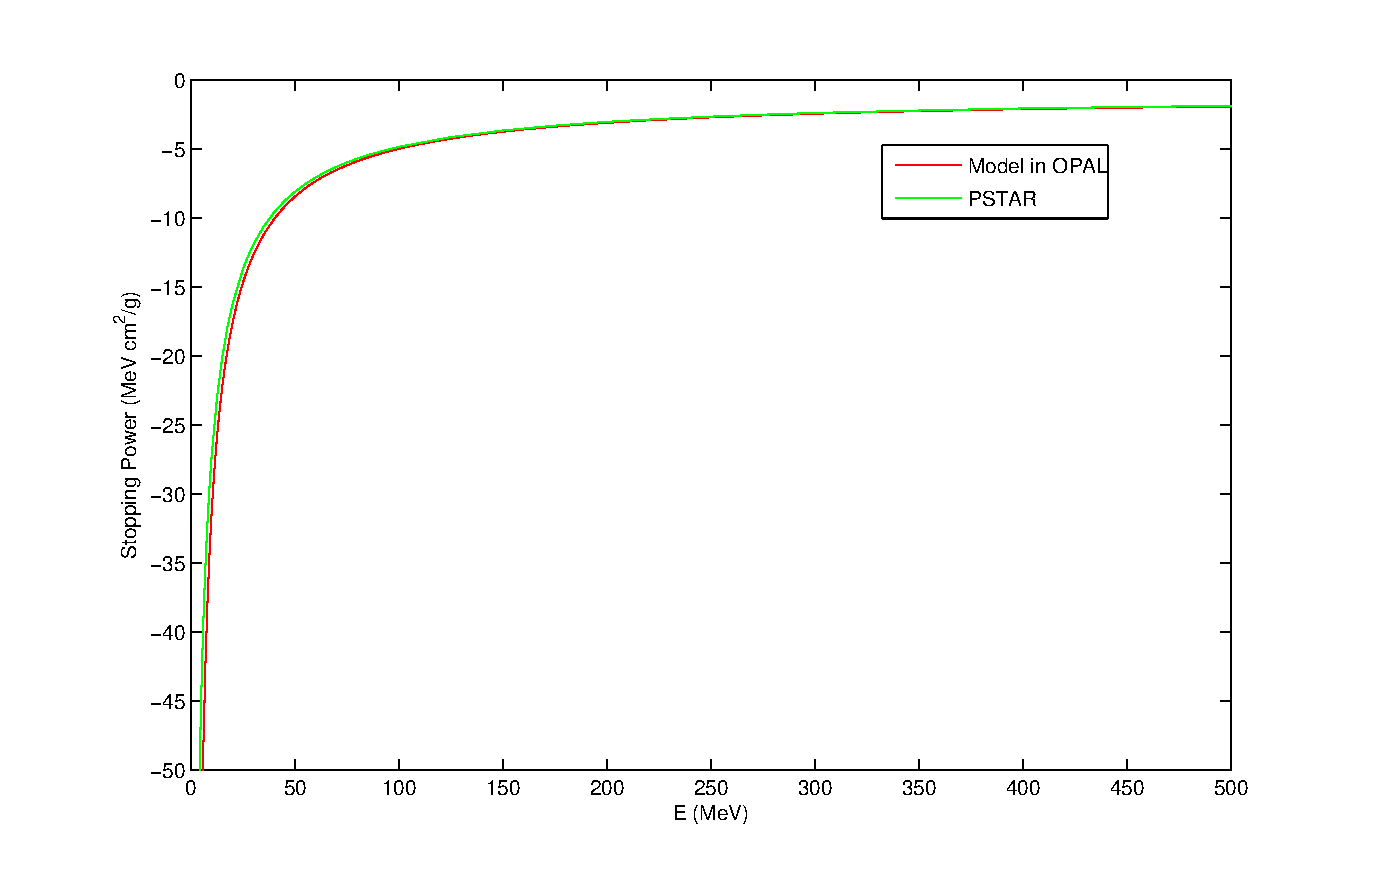
\includegraphics[width=0.5\textwidth]{figures/partmatter/dEdx}
\end{center}
\caption{The comparison of stopping power with PSTAR. }
\label{fig:dEdx}
\end{figure}

Energy straggling: For relatively thick absorbers such that the number of collisions is large, the energy loss distribution is shown to be Gaussian in form.
For non-relativistic heavy particles the spread $\sigma_0$ of the Gaussian distribution is calculated by:
\begin{equation}
\sigma_0^2=4\pi N_Ar_e^2(m_ec^2)^2\rho\frac{Z}{A}\Delta s,
\end{equation}
where $\rho$ is the density, $\Delta s$ is the thickness.

\section{The Coulomb Scattering}
The Coulomb scattering is treated as two independent events: the multiple Coulomb scattering and the large angle Rutherford scattering.\\
Using the distribution given in Classical Electrodynamics, by J. D. Jackson, the multiple- and single-scattering distributions can be written:
\begin{equation}
\label{eq:PM}
P_M(\alpha) \;\differential \alpha=\frac{1}{\sqrt{\pi}}e^{-\alpha^2}\;\differential\alpha,
\end{equation}
\begin{equation}
\label{eq:Ps}
P_S(\alpha) \;\differential{} \alpha=\frac{1}{8 \ln(204 Z^{-1/3})} \frac{1}{\alpha^3}\;\differential{}\alpha,
\end{equation}
where $\alpha=\frac{\theta}{<\Theta^2>^{1/2}}=\frac{\theta}{\sqrt 2 \theta_0}$.

\noindent The transition point is $\theta=2.5 \sqrt 2 \theta_0\approx3.5 \theta_0$,
\begin{equation}
\label{eq:Multiple}
\theta_0=\frac{\SI{13.6}{\mega\electronvolt}}{\beta c p} z \sqrt{\Delta s/X_0} [1+0.038 \ln(\Delta s/X_0)],
\end{equation}
where $p$ is the momentum, $\Delta s$ is the step size, and $X_0$ is the radiation length.

\subsection{Multiple Coulomb Scattering}
Generate two independent Gaussian random variables  with mean zero and variance one: $z_1$ and $z_2$.
If $z_2 \theta_0>3.5 \theta_0$, start over. Otherwise,
\begin{equation}
\label{eq:Multiplex}
x=x+\Delta s p_x+z_1 \Delta s \theta_0/\sqrt{12}+z_2 \Delta s \theta_0/2,
\end{equation}
\begin{equation}
\label{eq:Multiplepx}
p_x=p_x+z_2 \theta_0.
\end{equation}
Generate two independent Gaussian random variables  with mean zero and variance one: $z_3$ and $z_4$.
If $z_4 \theta_0>3.5 \theta_0$, start over. Otherwise,
\begin{equation}
\label{eq:Multipley}
y=y+\Delta s p_y+z_3 \Delta s \theta_0/\sqrt{12}+z_4 \Delta s \theta_0/2,
\end{equation}
\begin{equation}
\label{eq:Multiplepy}
p_y=p_y+z_4 \theta_0.
\end{equation}

\subsection{Large Angle Rutherford Scattering}

Generate a random number $\xi_1$, \textit{if} $\xi_1<\frac{\int_{2.5}^\infty P_S(\alpha)d\alpha}{\int_0^{2.5} P_M(\alpha)\;\differential\alpha+\int_{2.5}^\infty P_S(\alpha)\;\differential\alpha}=0.0047$, sampling the large angle
Rutherford scattering.\\
The cumulative distribution function of the large angle
Rutherford scattering is
\begin{equation}
\label{eq:Fa}
F(\alpha)=\frac{\int_{2.5}^\alpha P_S(\alpha) \;\differential \alpha}{\int_{2.5}^\infty P_S(\alpha) \;\differential \alpha}=\xi,
\end{equation}
where $\xi$ is a random variable. So
\begin{equation}
\label{eq:alpha}
\alpha=\pm 2.5 \sqrt{\frac{1}{1-\xi}}=\pm 2.5 \sqrt{\frac{1}{\xi}}.
\end{equation}
Generate a random variable $P_3$,\\
\textit{if} $P_3>0.5$
\begin{equation}
   \theta_{Ru}=2.5 \sqrt{\frac{1}{\xi}} \sqrt{2}\theta_0,
\end{equation}
\textit{else}
\begin{equation}
       \theta_{Ru}=-2.5 \sqrt{\frac{1}{\xi}} \sqrt{2}\theta_0.
\end{equation}

The angle distribution after Coulomb scattering is shown in \figref{Coulomb}.
The line is from Jackson's formula, and the points are simulations with Matlab.
For a thickness of $\Delta s=1e-4$ $m$, $\theta=0.5349 \alpha$ (in degree).

\begin{figure}[ht!]
\begin{center}
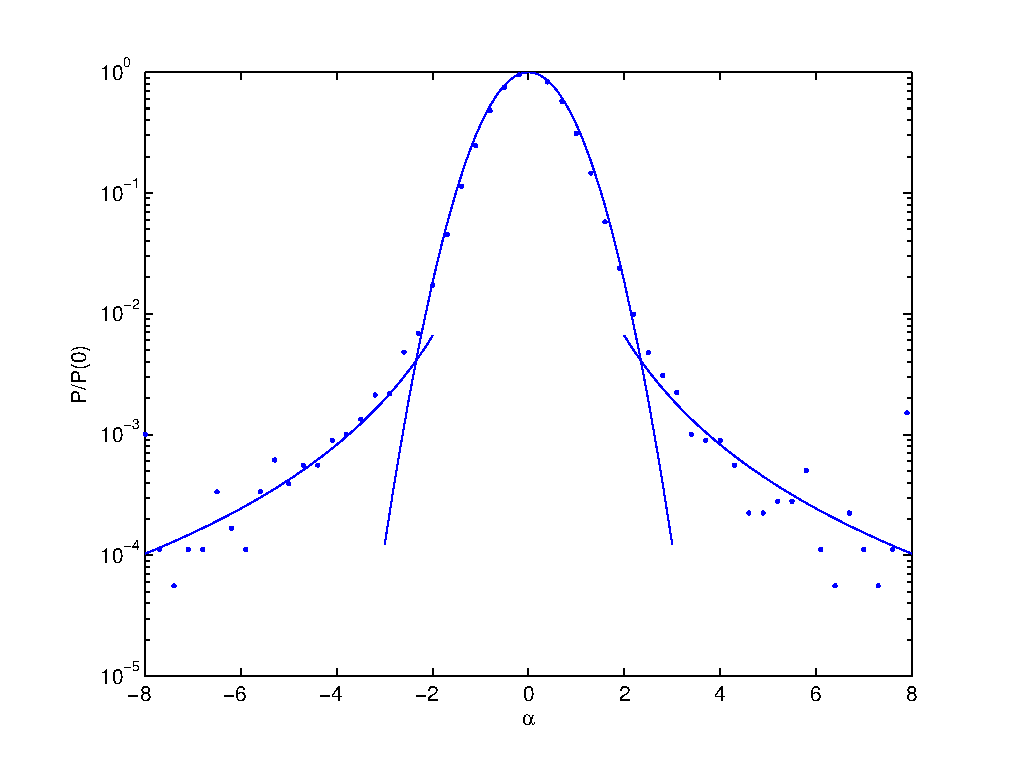
\includegraphics[width=.8\textwidth]{figures/partmatter/10steps}
\end{center}
\caption{The comparison of Coulomb scattering with Jackson's book. }
\label{fig:Coulomb}
\end{figure}

\section{The Flow Diagram of {\em CollimatorPhysics} Class in OPAL}
\begin{figure}[ht!]
\begin{center}
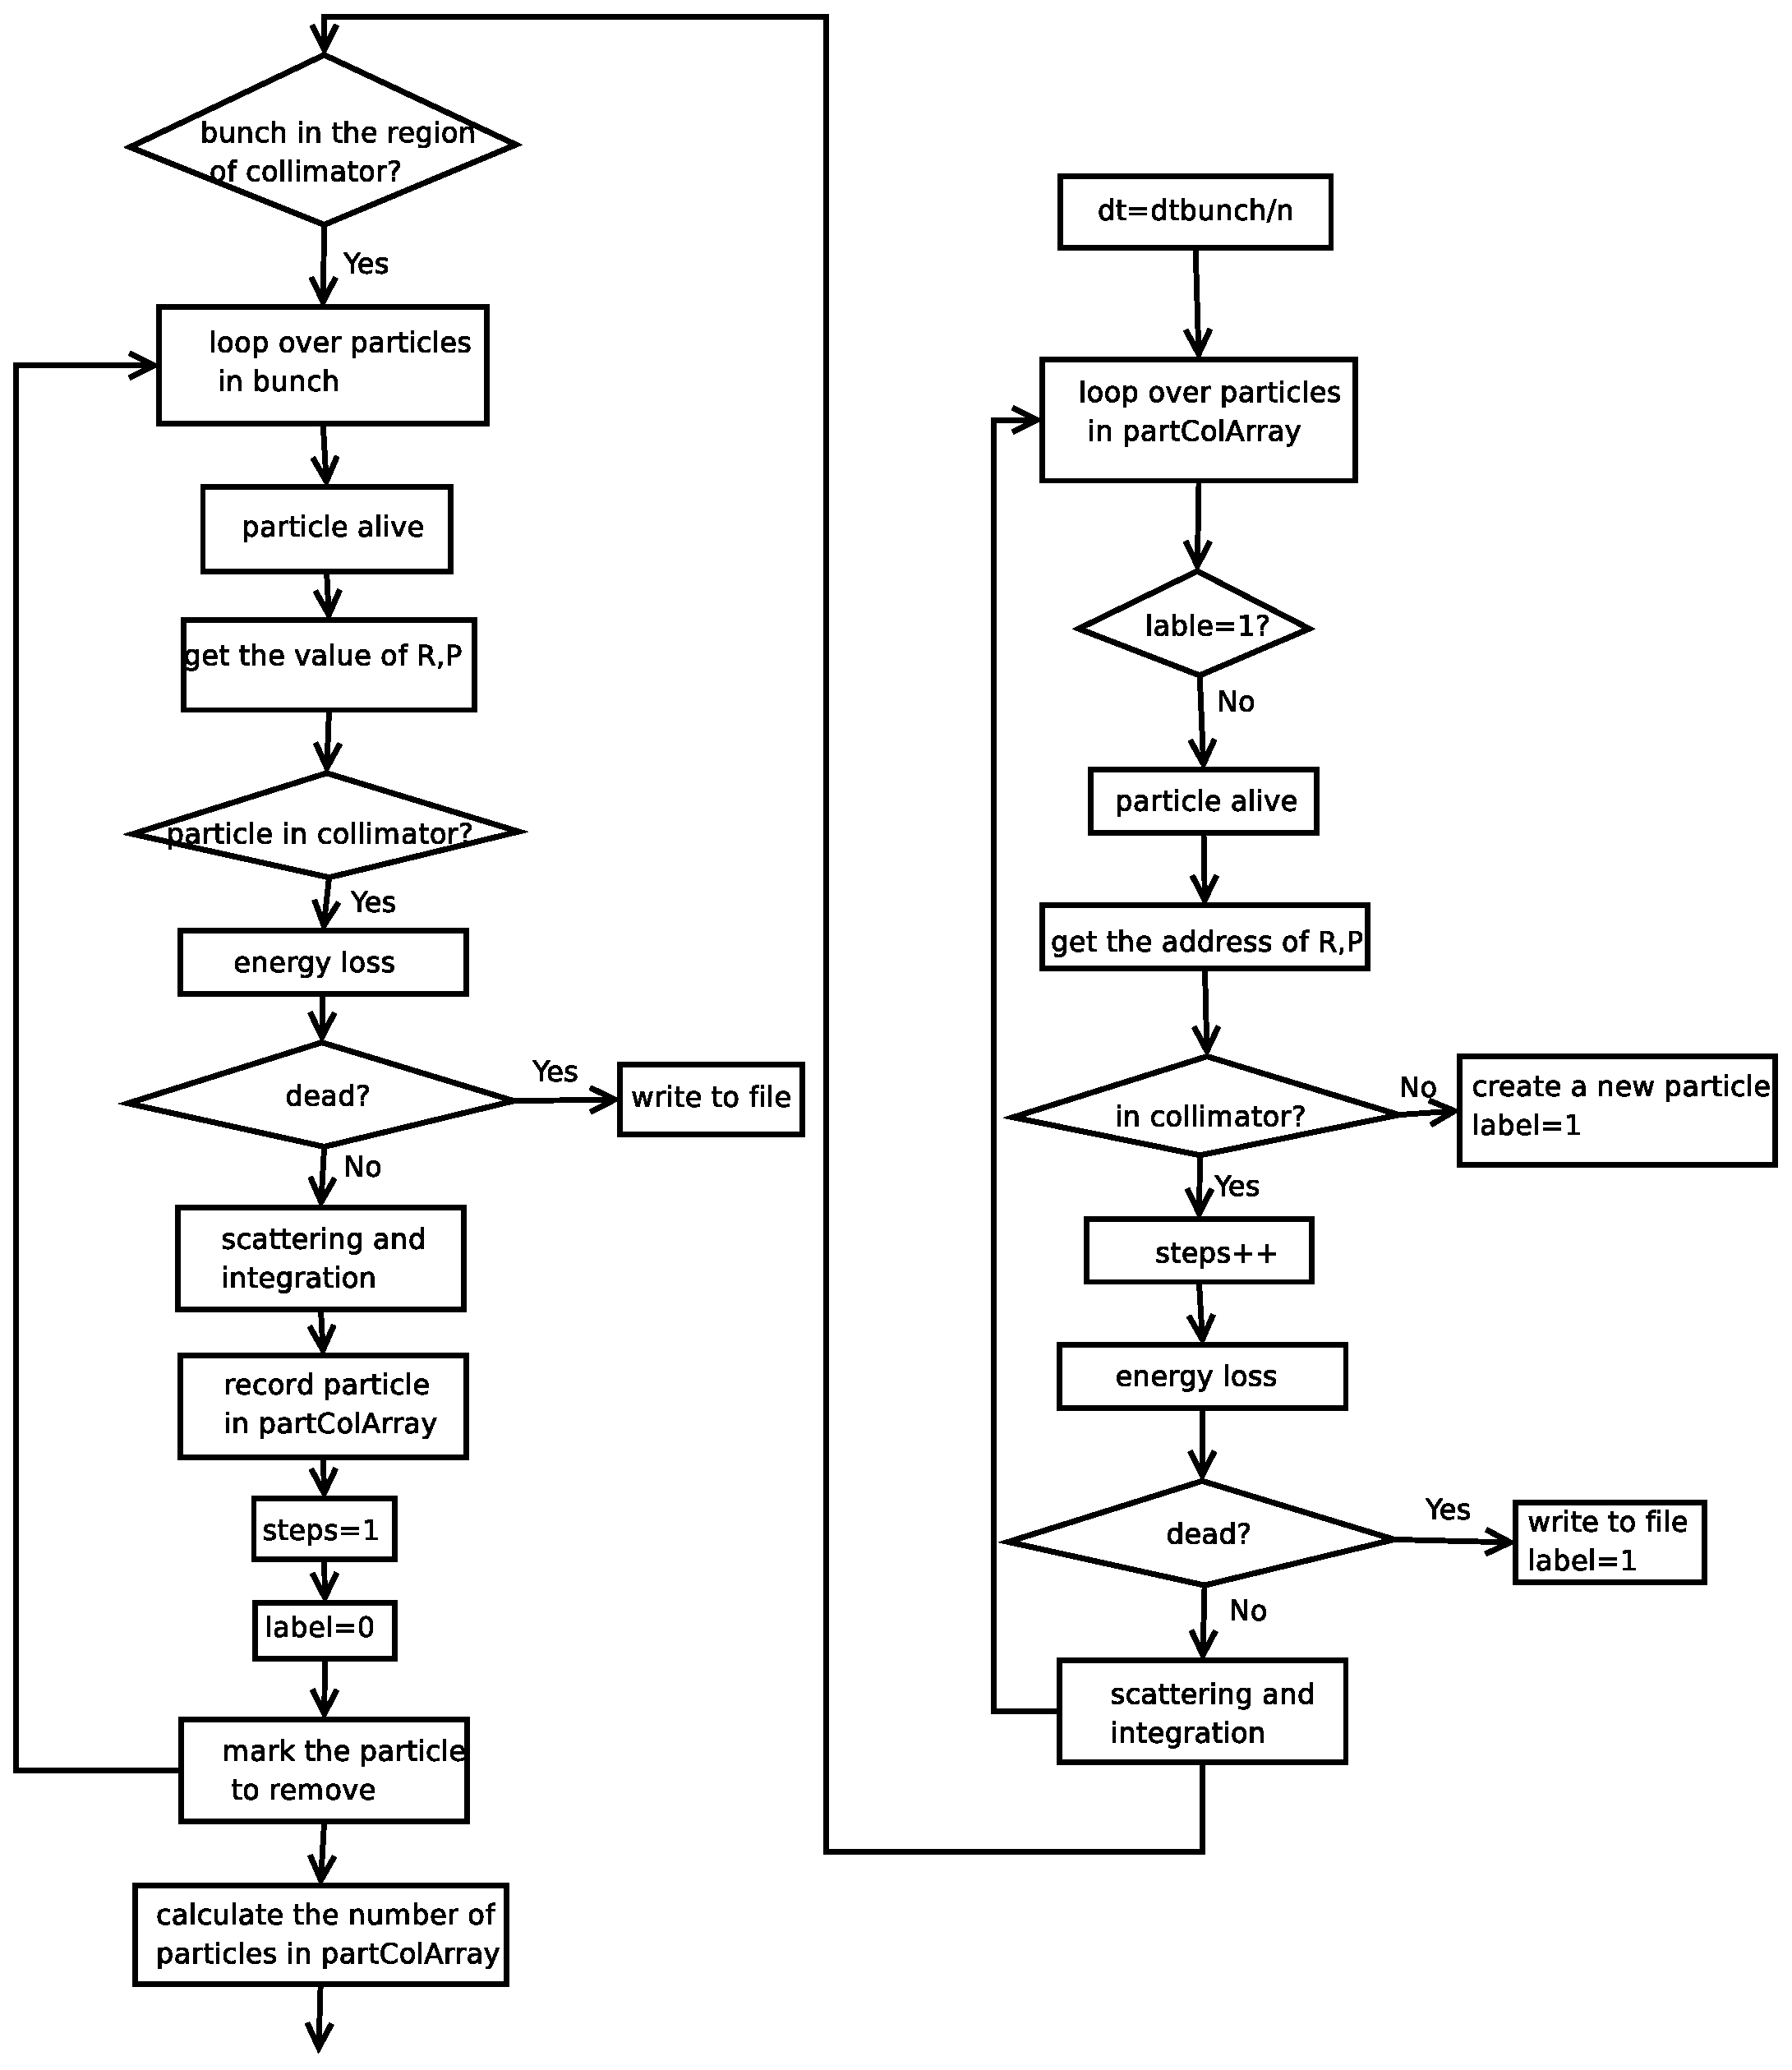
\includegraphics[width=0.8\textwidth]{figures/partmatter/diagram}
\end{center}
\caption{The diagram of CollimatorPhysics in \opal. }
\label{fig:diagram}
\end{figure}
\begin{figure}[ht!]
\begin{center}
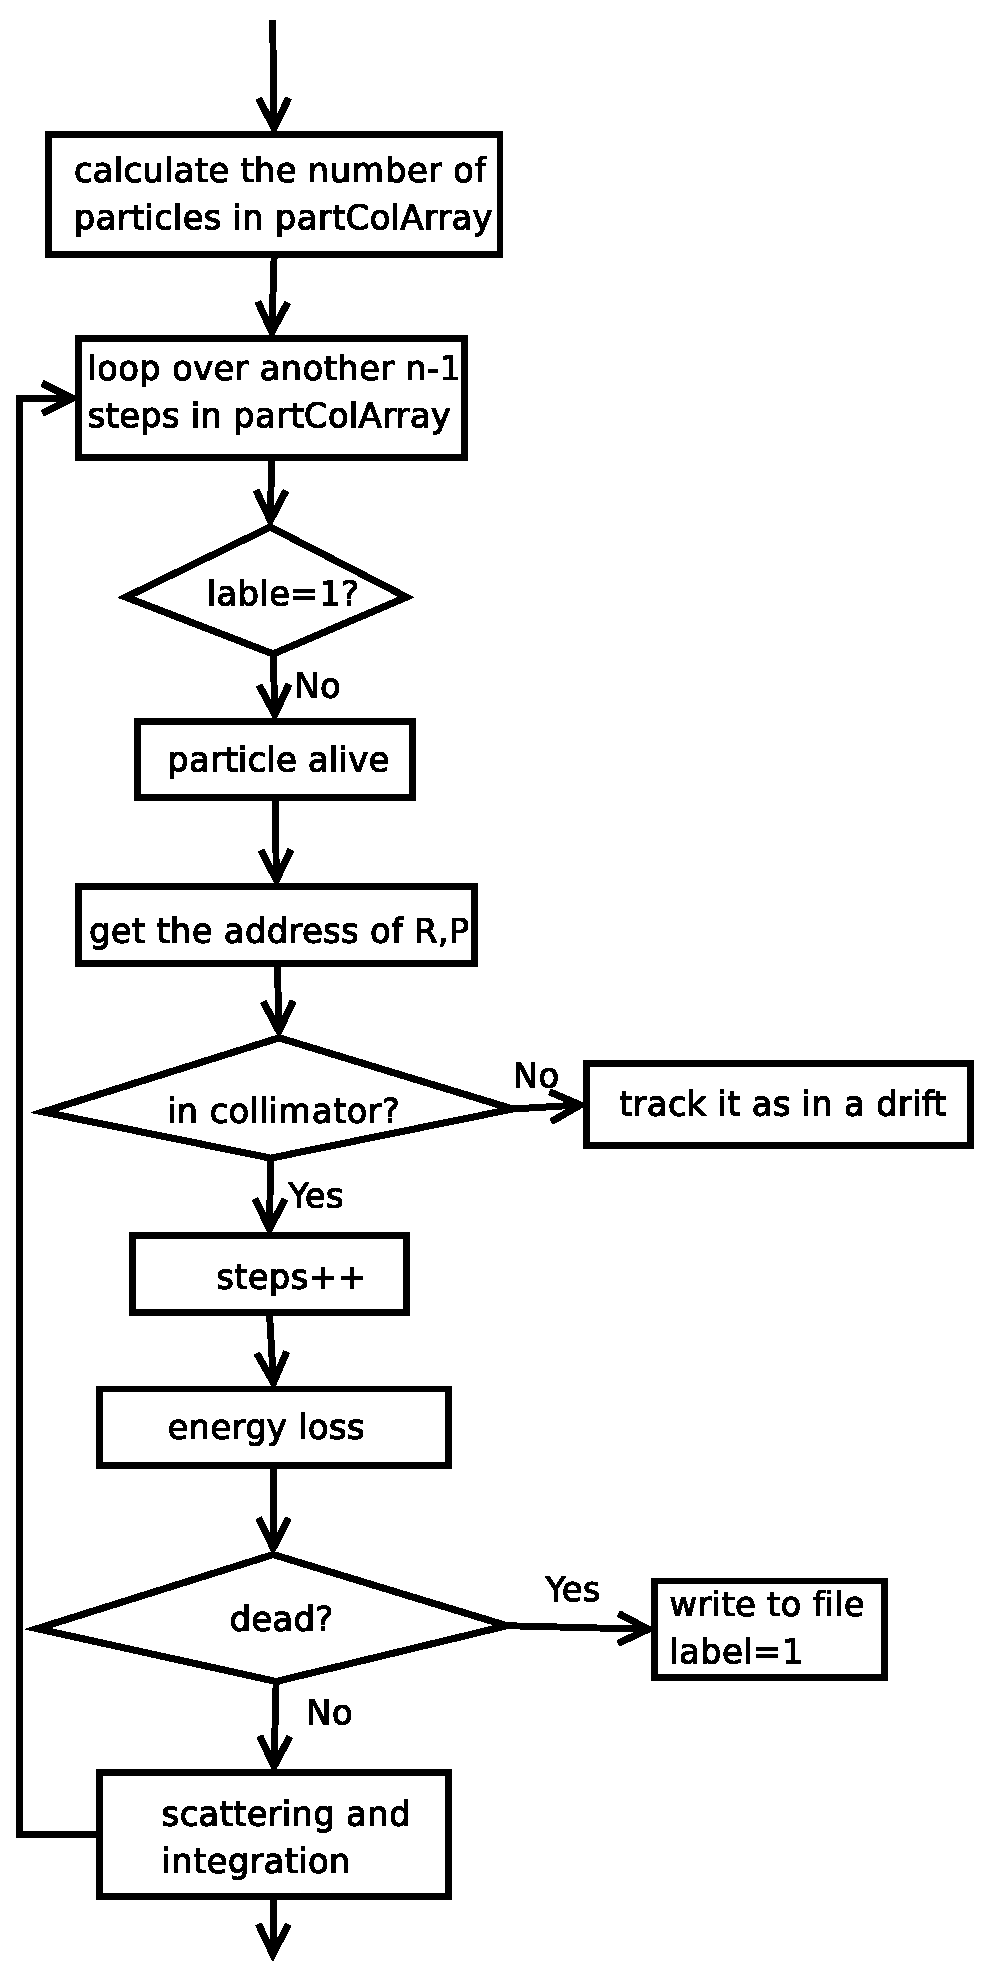
\includegraphics[width=0.6\textwidth]{figures/partmatter/Diagram2}
\end{center}
\caption{The diagram of CollimatorPhysics in \opal (continued). }
\label{fig:diagram2}
\end{figure}
\clearpage

\subsection{The Substeps}

Small step is needed in the routine of CollimatorPhysics.

If a large step is given in the main input file, in the file \filename{CollimatorPhysics.cpp},
it is divided by a integer number $n$ to make the step size using for the calculation of collimator physics less than 1.01e-12 s. As shown
by  \figref{diagram,diagram2} in the previous section, first we track one step for the particles already in the
collimator and the newcomers, then another (n-1) steps to make sure the particles in the collimator experience the same time as the ones
in the main bunch.

Now, if the particle leave the collimator during the  (n-1) steps, we track it as in a drift and put it back to the main bunch when
finishing (n-1) steps.

\section{Available Materials in \opal}
\begin{table}[H]\footnotesize
\centering
  \caption{List of materials with their parameters implemented in \opal.}
  \label{table:Materials}
  \begin{tabular}{|c|c|c|c|c|c|c|c|c|c|}
  \hline
  \tabhead{Material     & Z    &    A         &    $\rho$  [$g/cm^3$]     &    X0      [$g/cm^2$]     &    A2    &    A3    &    A4    &    A5 & \opal Name}
    \hline
    Aluminum        &    13        &          26.98        &              2.7        &    24.01        &    4.739        &    2766        &    164.5        &    2.023E-02 & \keyword{Aluminum }\\
    %\hline
    AluminaAl2O3        &    50        &          101.96        &              3.97        &    27.94        &    7.227        &    11210        &    386.4        &    4.474e-3 & \keyword{AluminaAl2O3 }\\
    %\hline
    Copper            &    29        &      63.54        &        8.96        &    12.86        &     4.194        &    4649        &    81.13        &    2.242E-02 & \keyword{Copper}\\
    %\hline
    Graphite            &    6        &       12.0172            &           2.210    &    42.7            &    2.601        &    1701        &    1279        &    1.638E-02 & \keyword{Graphite }\\
    %\hline
    GraphiteR6710        &    6        &       12.0172            &           1.88        &    42.7            &    2.601        &    1701        &    1279        &    1.638E-02 & \keyword{GraphiteR6710}\\
    %\hline
    Titan            &    22        &      47.8        &          4.54        &    16.16        &    5.489        &    5260        &    651.1        &    8.930E-03 & \keyword{Titan }\\
    %\hline
    Air                &    7        &    14            &        0.0012        &    37.99        &    3.350        &    1683        &    1900        &    2.513E-02 & \keyword{Air }\\
    %\hline
    Kapton            &    6        &    12            &    1.4            &    39.95        &    2.601        &    1701        &    1279        &    1.638E-02 & \keyword{Kapton }\\
    %\hline
    Gold                &    79        &    197            &    19.3            &    6.46            &    5.458        &    7852        &    975.8        &    2.077E-02 & \keyword{Gold }\\
    %\hline
    Water            &    10        &    18            &    1            &    36.08        &    2.199        &    2393        &    2699        &    1.568E-02 & \keyword{Water }\\
    %\hline
    Mylar            &    6.702    &    12.88            &    1.4            &    39.95        &    3.35        &    1683        &    1900        &     2.513E-02 & \keyword{Mylar }\\
    %\hline
    Berilium                 &    4        &    9.012        &    1.848        &    65.19        &    2.590        &    966.0        &    153.8        &     3.475E-02 & \keyword{Berilium }\\
    %\hline
    Molybdenum                &    42        &    95.94        &    10.22        &    9.8            &    7.248        &    9545        &    480.2        &     5.376E-03 &  \keyword{Molybdenum}\\
    \hline
    \end{tabular}
\end{table}



\section{Example of an Input File}

\examplefromfile{examples/particlematterinteraction.in}

FX5 is a slit in x direction, the  \keyword{APERTURE} is \textbf{POSITIVE}, the first value in  \keyword{APERTURE} is the left part, the second value is the right part.
FX16 is a slit in y direction,  the  \keyword{APERTURE} is \textbf{NEGATIVE}, the first value in  \keyword{APERTURE} is the down part, the second value is the up part.

\section{A Simple Test}
A cold Gaussian beam with $\sigma_x=\sigma_y=5$ mm.
The position of the  collimator is from 0.01 m to 0.1 m, the half aperture in y direction is $3$ mm.  \figref{longcoll}
shows the trajectory of particles which are either absorbed or deflected by a copper slit. As a benchmark of the collimator model in \opal, \figref{Espectrum} shows the energy spectrum  and angle deviation at z=0.1 m after an elliptic collimator.
\begin{figure}[ht!]
\begin{center}
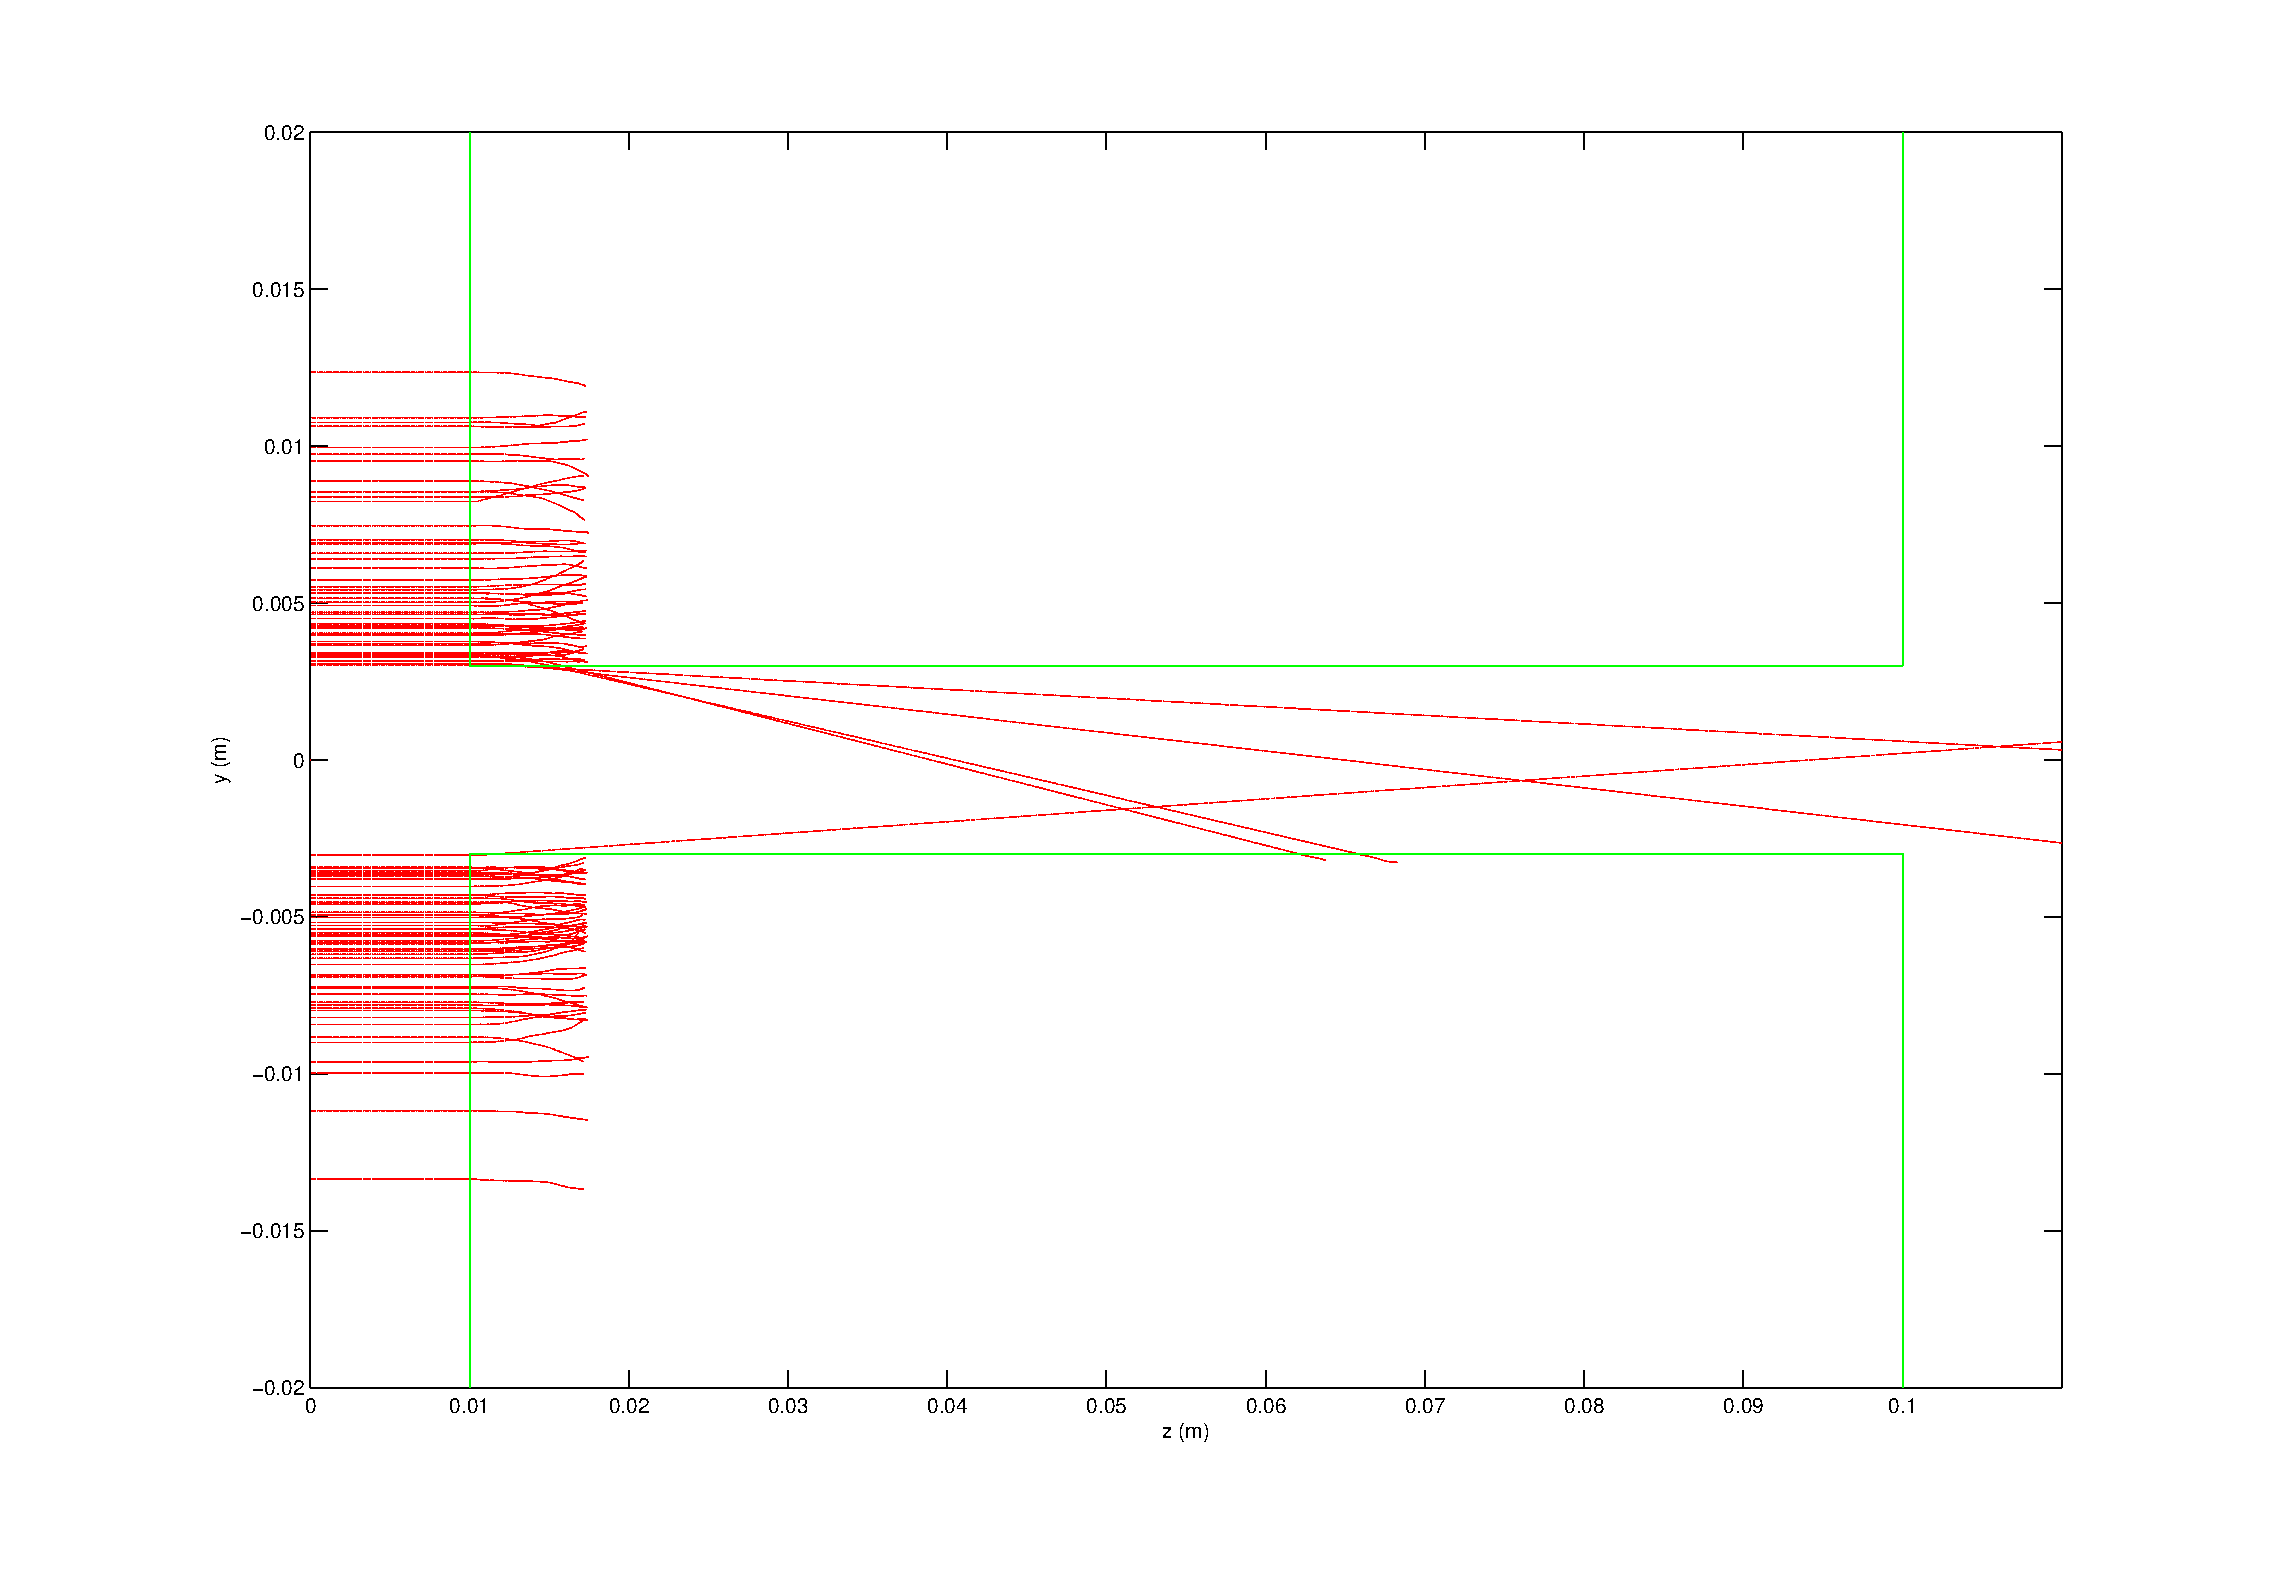
\includegraphics[width=0.8\textwidth]{figures/partmatter/longcoll6}
\end{center}
\caption{The passage of protons through the collimator. }
\label{fig:longcoll}
\end{figure}

\begin{figure}[ht!]
\begin{center}
\includegraphics[width=0.8\textwidth]{figures/partmatter/spectandscatter}
\end{center}
\caption{The energy spectrum and scattering angle at z=0.1 m}
\label{fig:Espectrum}
\end{figure}

%----------- Footer control ------------------
\ifthenelse{\boolean{FullOPALManual}}
{
  %do nothing
}
% else (for individual document creation)
{
\appendix
\printbibliography
\end{document}
}
%---------------------------------------------